\documentclass[12pt,a4paper]{article}
\usepackage[latin1]{inputenc}
\usepackage[english]{babel}
\usepackage{amsmath}
\usepackage{amsfonts}
\usepackage{amssymb}
\usepackage{makeidx}
\usepackage{graphicx}
\usepackage{float}
\usepackage{comment}
\usepackage{caption}
\usepackage{subcaption}

\usepackage{lmodern}
\usepackage[left=2cm,right=2cm,top=2cm,bottom=2cm]{geometry}
\author{Mads Kristensen}
\begin{document}

%\chapter{Results of model training and testing}
This chapter will present the results from training and testing of the three data representations. Training results support arguments to how optimization of the models were performed as well as the generalization performance of the models. Final testing shows how the trained model will generalize unseen data, displayed in a confusion matrix, along with it's calculated type 1 and type 2 errors. 

\section{Initial optimization and training of the models}
Initial grid search of hyperparameters led to results that were used as an indication to initial setting of the models in order to (improve) raise or maintain performance for the different networks. The results of the grid search is shown in %\autoref{tab:gridResults}. 


\section{Training optimization based on validation performance}
Further optimization was performed based the development in validation performance. These results were used to evaluate the performance of the model, in terms of the under- and overfitting of the training subset. The results of this training optimization process is shown as graphs in %\autoref{fig:}

\subsection{Simple representation training results}
\begin{figure} [H]
\centering

\includegraphics[width=0.2\textwidth]{figures/missimage}
\caption{Training graphs: }
\label{fig:simpleGraph}  
\end{figure}

\begin{table}[H]
\centering
\begin{tabular}{|p{2cm}|p{2.2cm}|p{2.2cm}|p{2.2cm}|p{2cm}|p{2cm}|}
\hline
\textbf{Classes}          & \textbf{Avg. Accuracy (\%)} & \textbf{Avg. Sensitvity (\%)} & \textbf{Avg. Specificity (\%)} & \textbf{Avg. PPV (\%)} & \textbf{Avg. NPV (\%)} \\ \hline
\textbf{Symptom Duration} & $54.56\%\newline(\pm12.81\%)$ & $50.68\%\newline(\pm0.15\%)$ & $59.55\%\newline(\pm0.15\%)$ & $58.33\%\newline(\pm0.25\%)$ & $51.33\%\newline(\pm0.20\%)$ \\ \hline
\textbf{Pain intensity}   & $63.33\%\newline(\pm1.67\%)$ & $0.00\%\newline(\pm0.00\%)$ & $63.33\%\newline(\pm0.02\%)$ & $0.00\%\newline(\pm0.00\%)$ & $100\%\newline(\pm0.00\%)$ \\ \hline
\end{tabular}
\label{my-label}
\caption{My caption}
\end{table}

\subsection{Binary representation training results}
\begin{figure} [H]
\centering

\includegraphics[width=0.2\textwidth]{figures/missimage}
\caption{Training graphs:}
\label{fig:binaryGraph}  
\end{figure}

\begin{table}[H]
\centering
\begin{tabular}{|p{2cm}|p{2.2cm}|p{2.2cm}|p{2.2cm}|p{2cm}|p{2cm}|}
\hline
Classes          & Mean Accuracy (\%) & Mean Sensitvity (\%) & Mean Specificity (\%) & Mean PPV (\%) & Mean NPV (\%) \\ \hline
Symptom Duration & $59.51\%\newline(\pm11.20\%)$ & $62.16\%\newline(\pm21.59\%)$ & $62.20\%\newline(\pm18.13\%)$ & $54.53\%\newline(\pm27.10\%)$ & $69.10\%\newline(\pm19.47\%)$ \\ \hline
Pain intensity   & $65.04\%\newline(\pm10.83\%)$ & $48.23\%\newline(\pm0.28\%)$ & $71.02\%\newline(\pm0.12\%)$ & $44.09\%\newline(\pm0.26\%)$ & $78.65\%\newline(\pm0.14\%)$ \\ \hline
\end{tabular}
\label{my-label}
\caption{My caption}
\end{table}

\subsection{Combined representation training results}
\begin{figure} [H]
\centering

\includegraphics[width=0.2\textwidth]{figures/missimage}
\caption{Training graphs:}
\label{fig:combinedGraph}  
\end{figure}

\begin{table}[H]
\centering
\begin{tabular}{|p{2cm}|p{2.2cm}|p{2.2cm}|p{2.2cm}|p{2cm}|p{2cm}|}
\hline
Classes          & Mean Accuracy (\%) & Mean Sensitvity (\%) & Mean Specificity (\%) & Mean PPV (\%) & Mean NPV (\%) \\ \hline
Symptom Duration & $55.49\%\newline(\pm10.06\%)$ & $55.23\%\newline(\pm16.07\%)$ & $56.99\%\newline(\pm12.55\%)$ & $42.92\%\newline(\pm21.03\%)$ & $68.47\%\newline(\pm13.90\%)$ \\ \hline
Pain intensity   & $65.14\%\newline(\pm12.87\%)$ & $37.50\%\newline(\pm0.35\%)$ & $67.34\%\newline(\pm0.15\%)$ & $22.14\%\newline(\pm0.20\%)$ & $92.41\%\newline(\pm0.07\%)$ \\ \hline
\end{tabular}
\label{my-label}
\caption{My caption}
\end{table}




\section{Testing results}
These result reflect the generalization performance of the three representation models, to which the models classification capabilities to unseen data is shown in confusion matrices, from where a type 1 and type 2 error is calculated. 


\subsection{Simple representation training results}

\begin{figure}[H]
  \begin{subfigure}[b]{0.45\textwidth}
    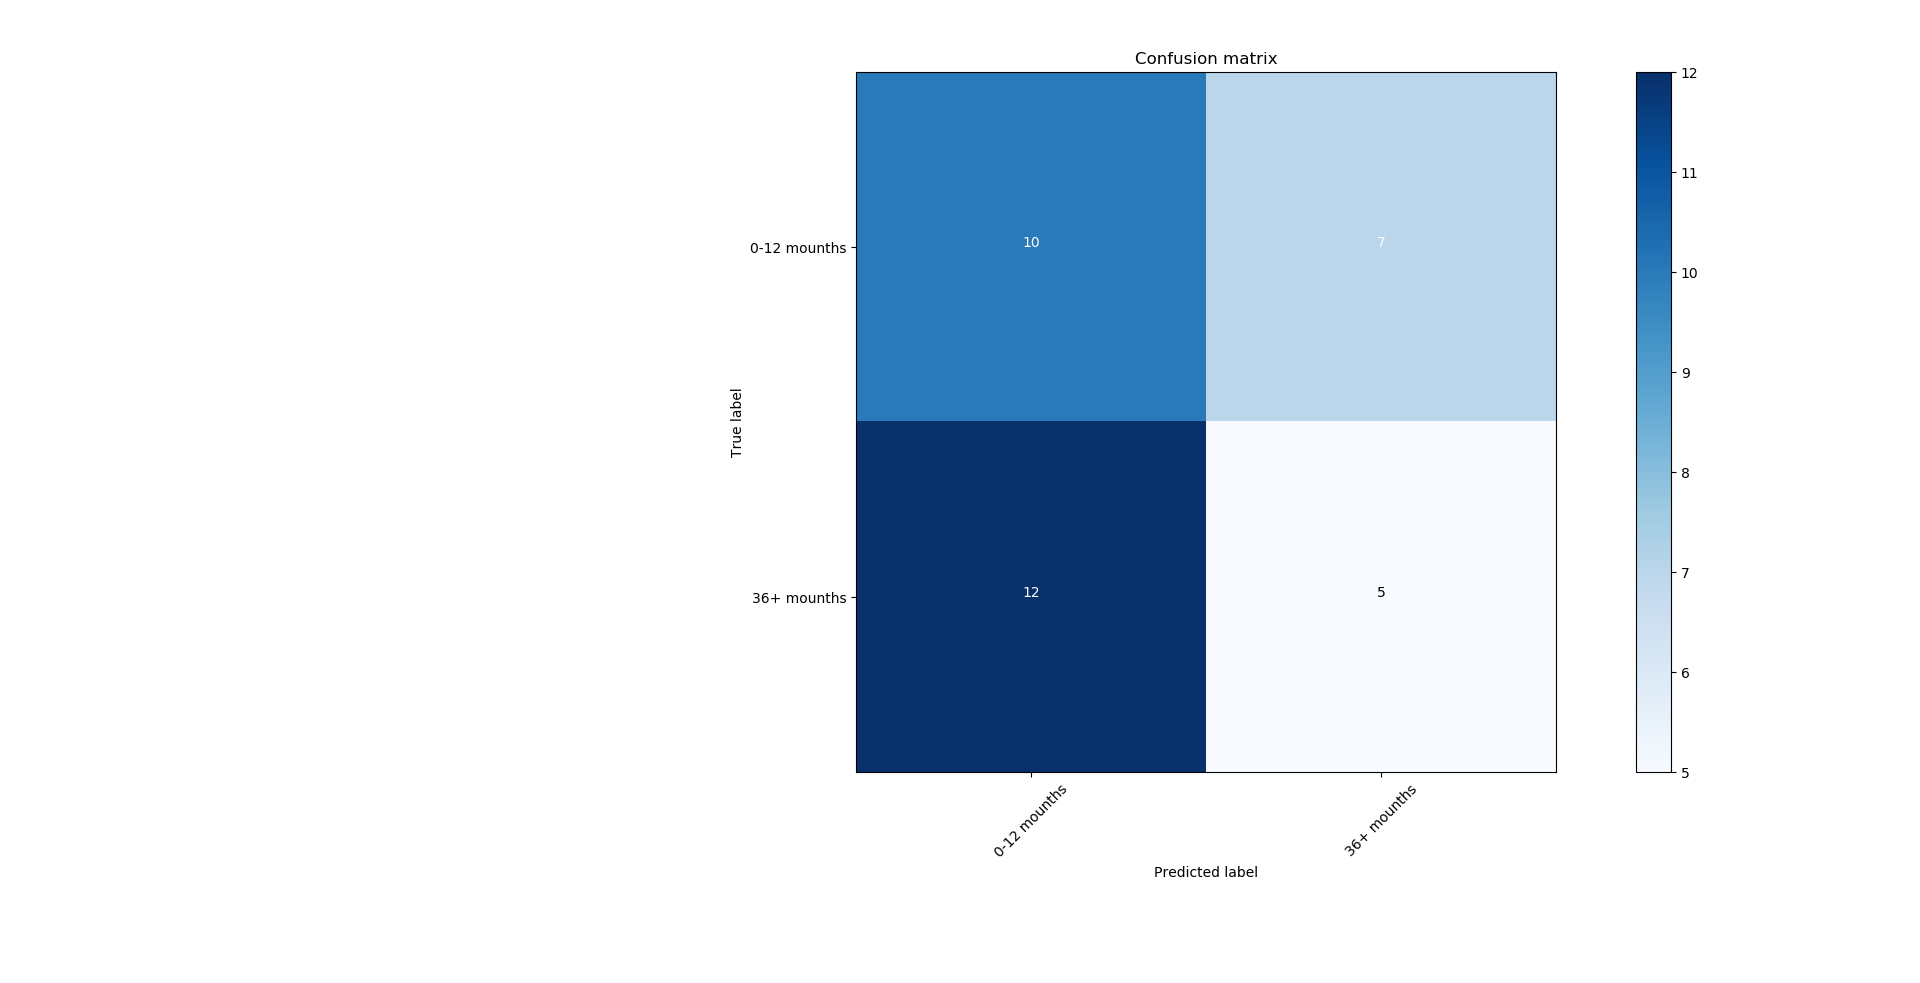
\includegraphics[width=\textwidth]{figures/sdura2cla}
    \caption{Confusion matrix for classification of symptom duration}
    \label{fig:f1}
  \end{subfigure}
  \hfill
  \begin{subfigure}[b]{0.45\textwidth}
    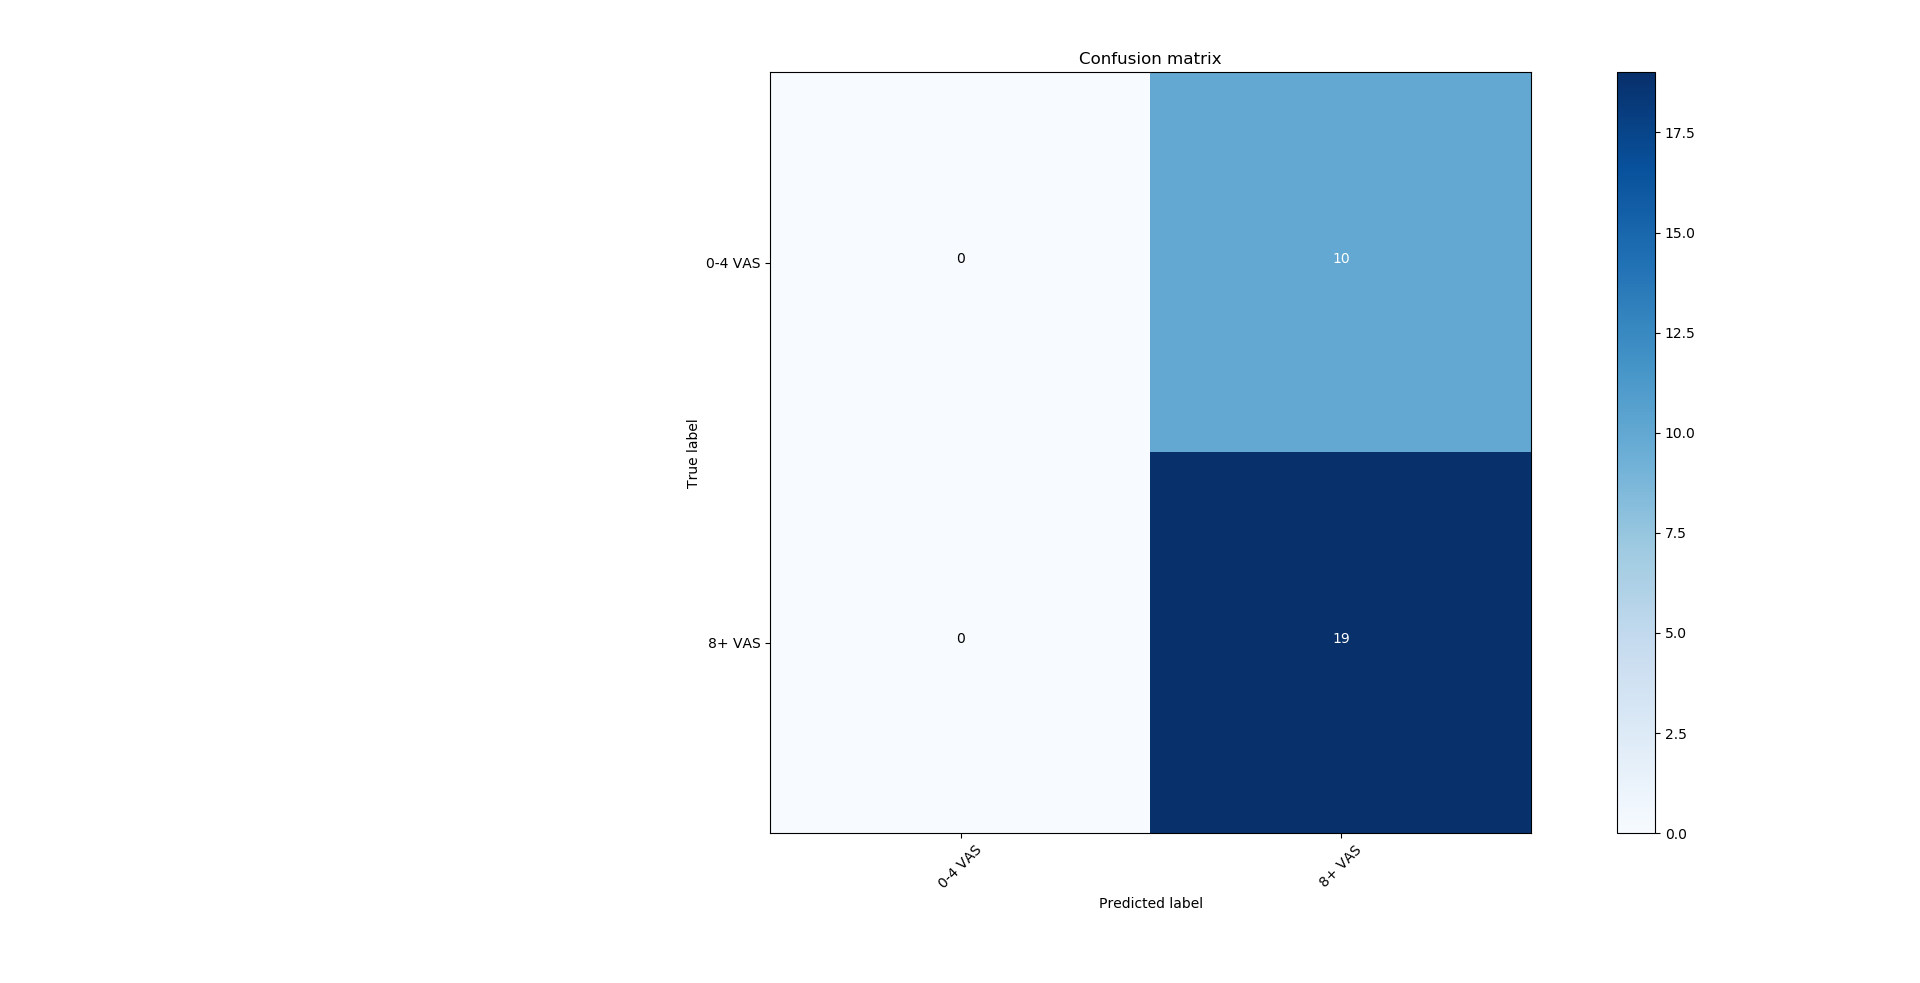
\includegraphics[width=\textwidth]{figures/spain2cla}
    \caption{Confusion matrix for classification of pain intensity}
    \label{fig:f2}
  \end{subfigure}
  \caption{Confusion matrices for simple representation testing}
\end{figure}


\begin{table}[H]
\centering
\begin{tabular}{|p{2cm}|p{2.2cm}|p{2.2cm}|p{2.2cm}|p{2cm}|p{2cm}|}
\hline
Classes          & Accuracy (\%) & Sensitivity (\%) & Specificity (\%) & PPV (\%) & NPV (\%) \\ \hline
Symptom Duration &                    &                      &                       &               &               \\ \hline
Pain intensity   &                    &                      &                       &               &               \\ \hline
\end{tabular}
\label{my-label}
\caption{My caption}
\end{table}


\subsection{Binary representation training results}

\begin{figure}[H]
  \begin{subfigure}[b]{0.45\textwidth}
    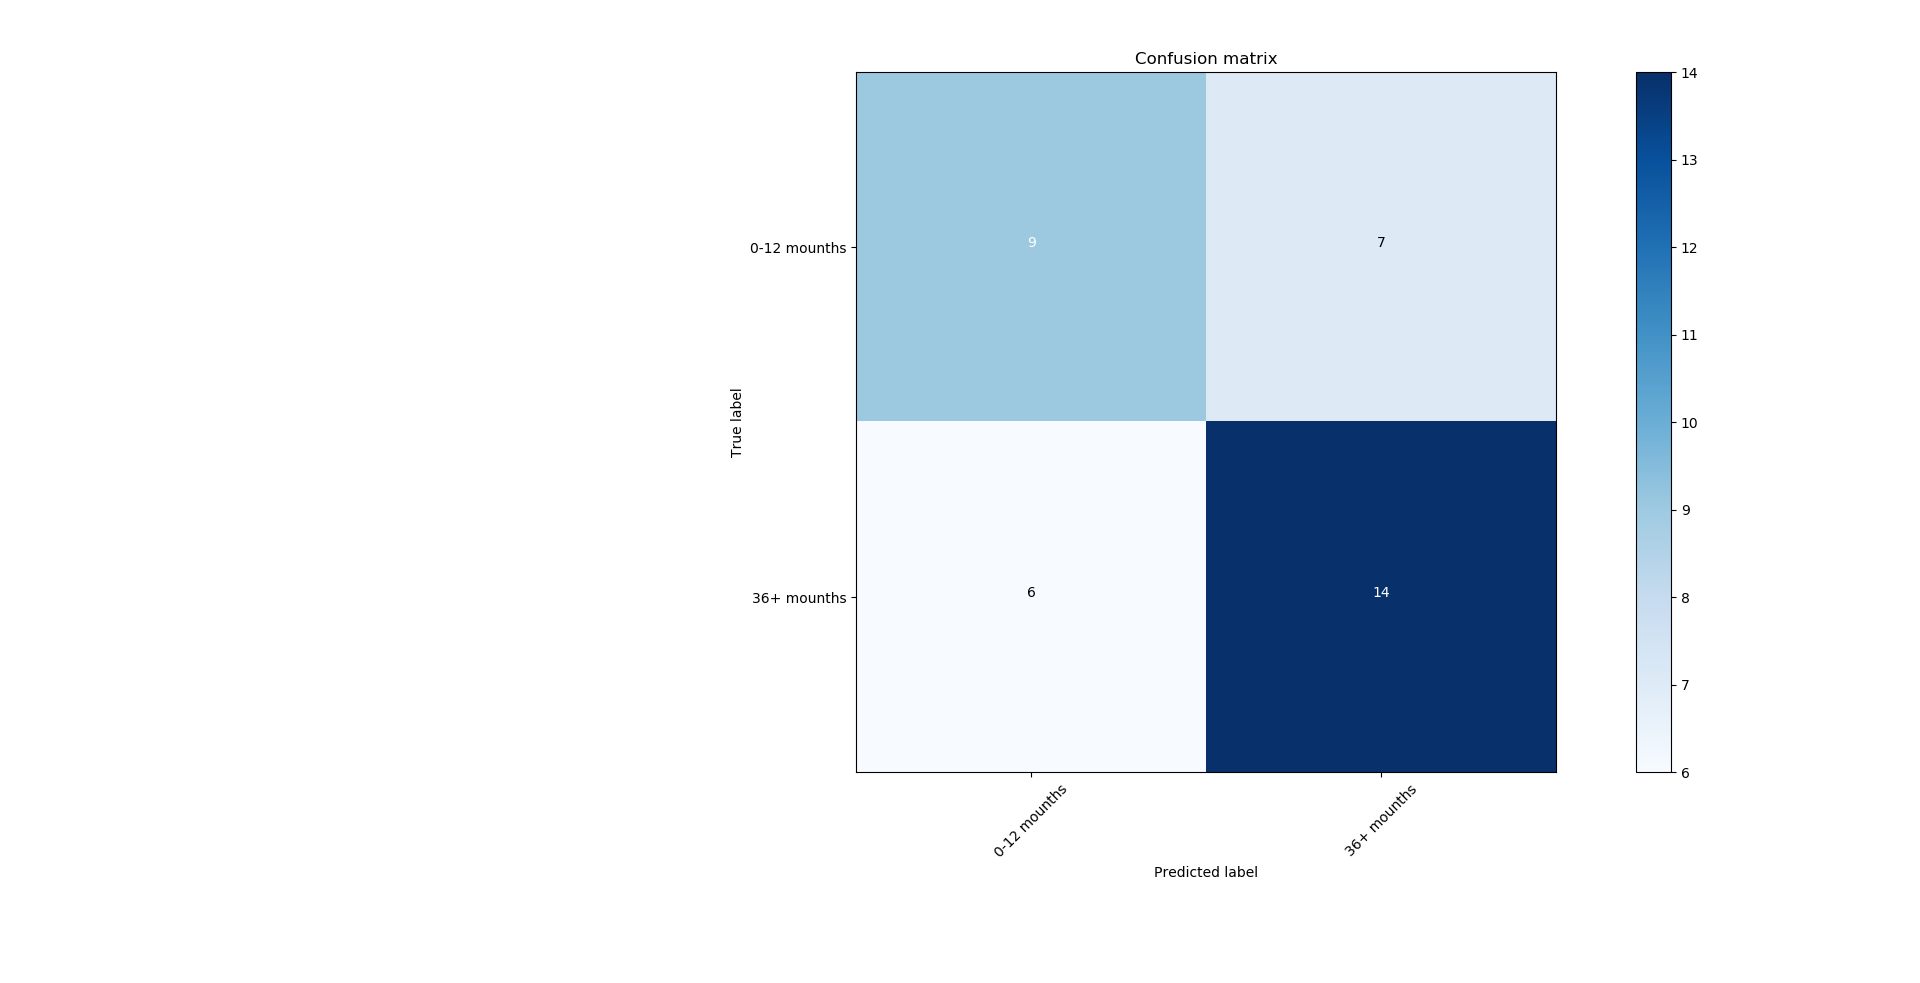
\includegraphics[width=\textwidth]{figures/bdura2cla}
    \caption{Confusion matrix for classification of symptom duration}
    \label{fig:f11}
  \end{subfigure}
  \hfill
  \begin{subfigure}[b]{0.45\textwidth}
    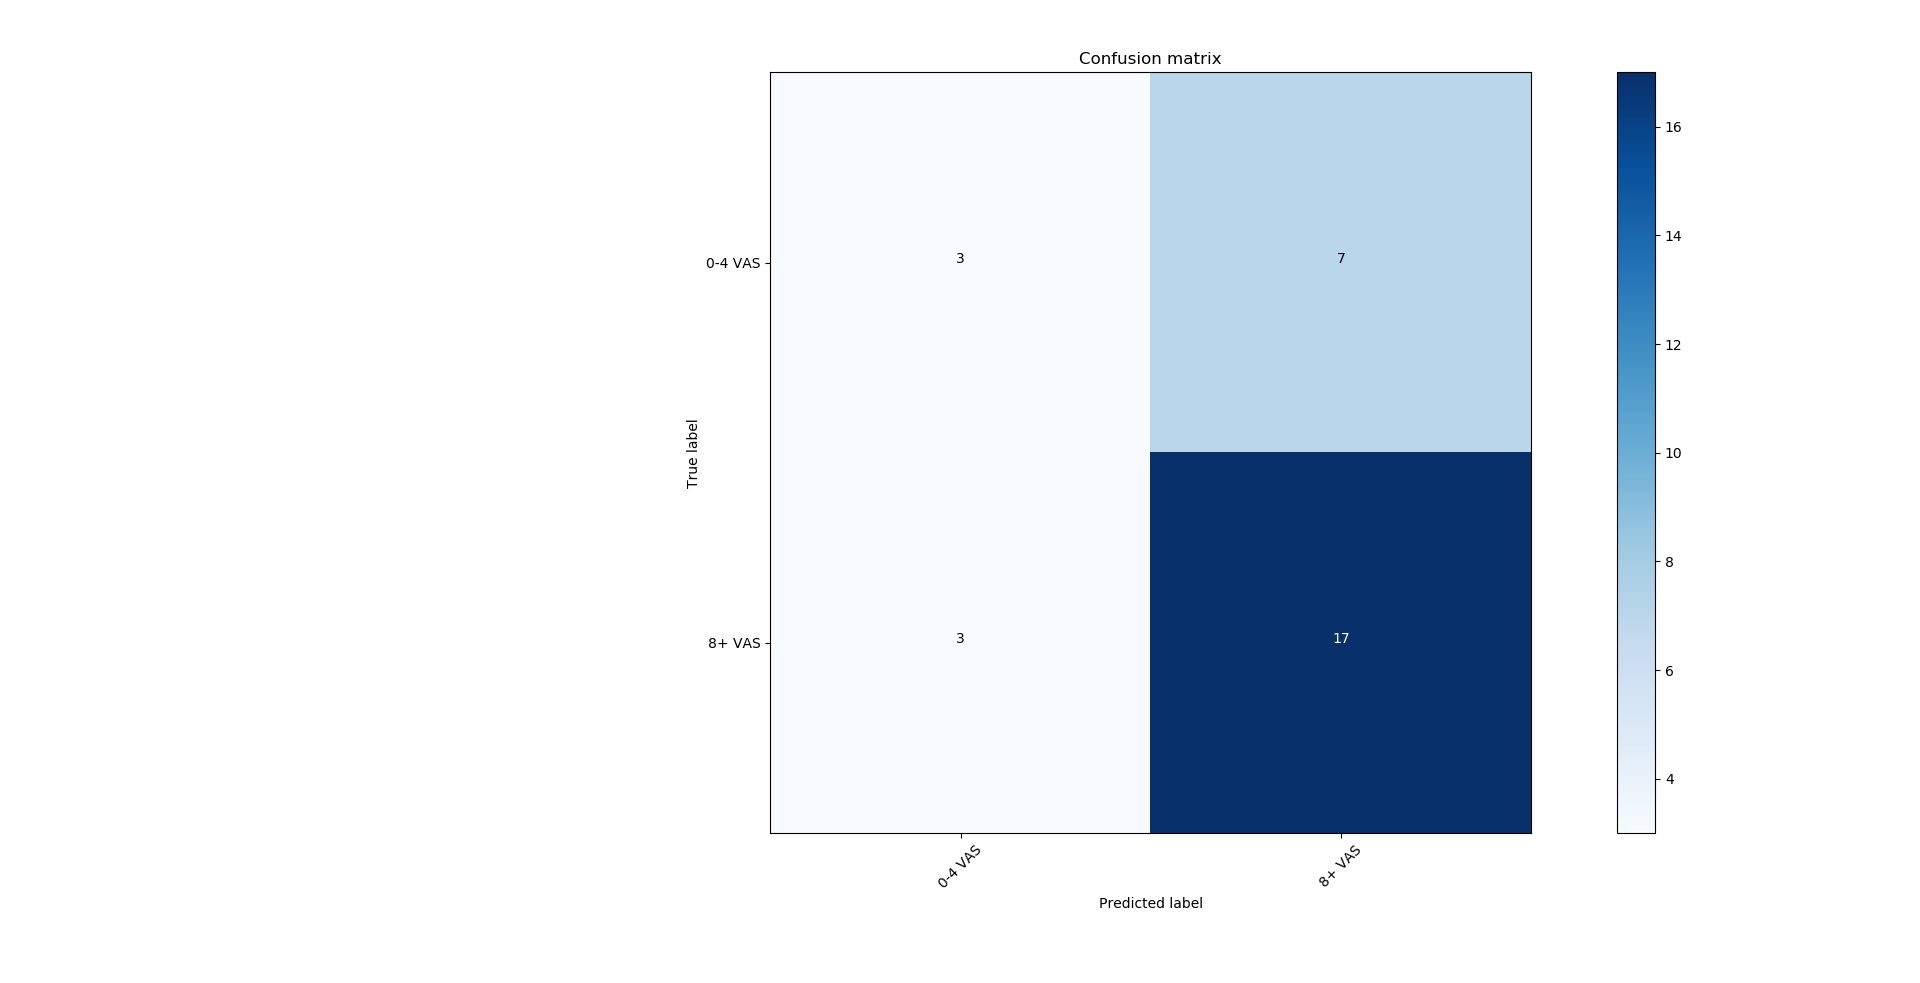
\includegraphics[width=\textwidth]{figures/bpain2cla}
    \caption{Confusion matrix for classification of pain intensity}
    \label{fig:f22}
  \end{subfigure}
  \caption{Confusion matrices for binary representation testing}
\end{figure}



\begin{table}[H]
\centering
\begin{tabular}{|p{2cm}|p{2.2cm}|p{2.2cm}|p{2.2cm}|p{2cm}|p{2cm}|}
\hline
Classes          & Accuracy (\%) & Sensitivity (\%) & Specificity (\%) & PPV (\%) & NPV (\%) \\ \hline
Symptom Duration &                    &                      &                       &               &               \\ \hline
Pain intensity   &                    &                      &                       &               &               \\ \hline
\end{tabular}
\label{my-label}
\caption{My caption}
\end{table}



\subsection{Combined representation training results}

\begin{figure}[H]
  \begin{subfigure}[b]{0.45\textwidth}
    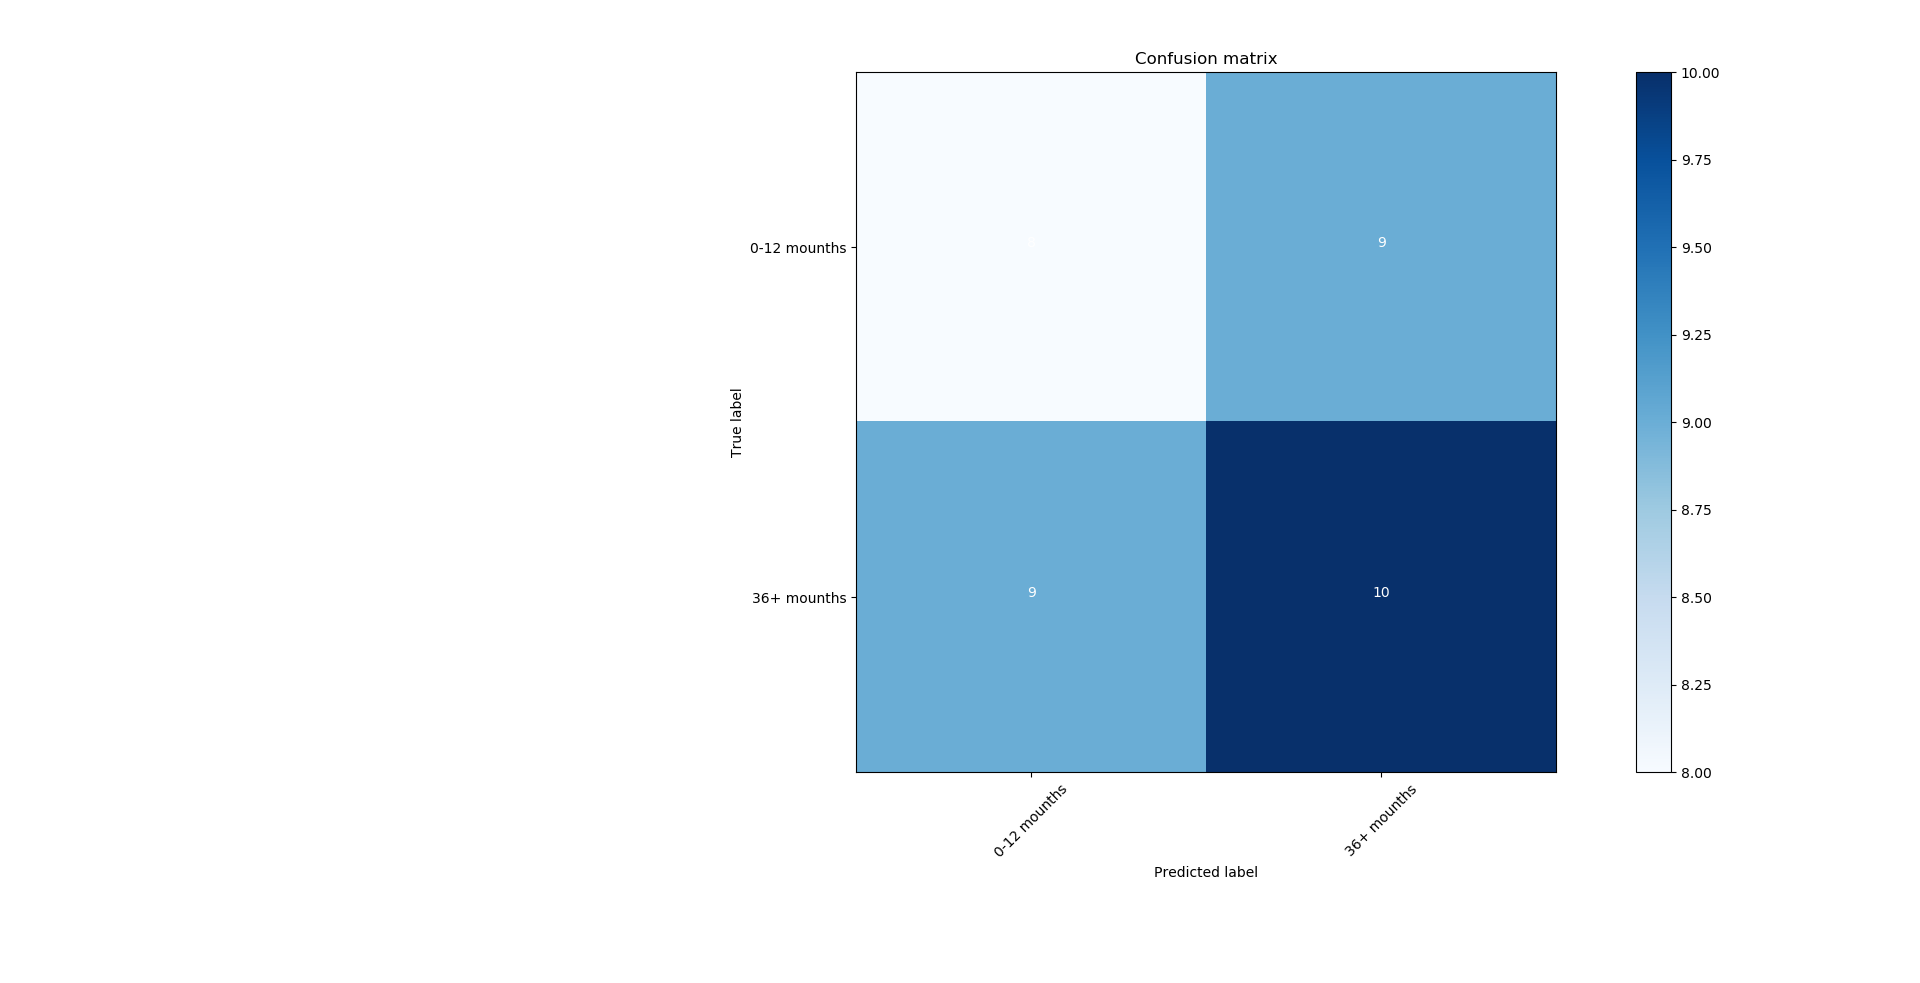
\includegraphics[width=\textwidth]{figures/edura2cla}
    \caption{Confusion matrix for classification of symptom duration}
    \label{fig:f1}
  \end{subfigure}
  \hfill
  \begin{subfigure}[b]{0.45\textwidth}
    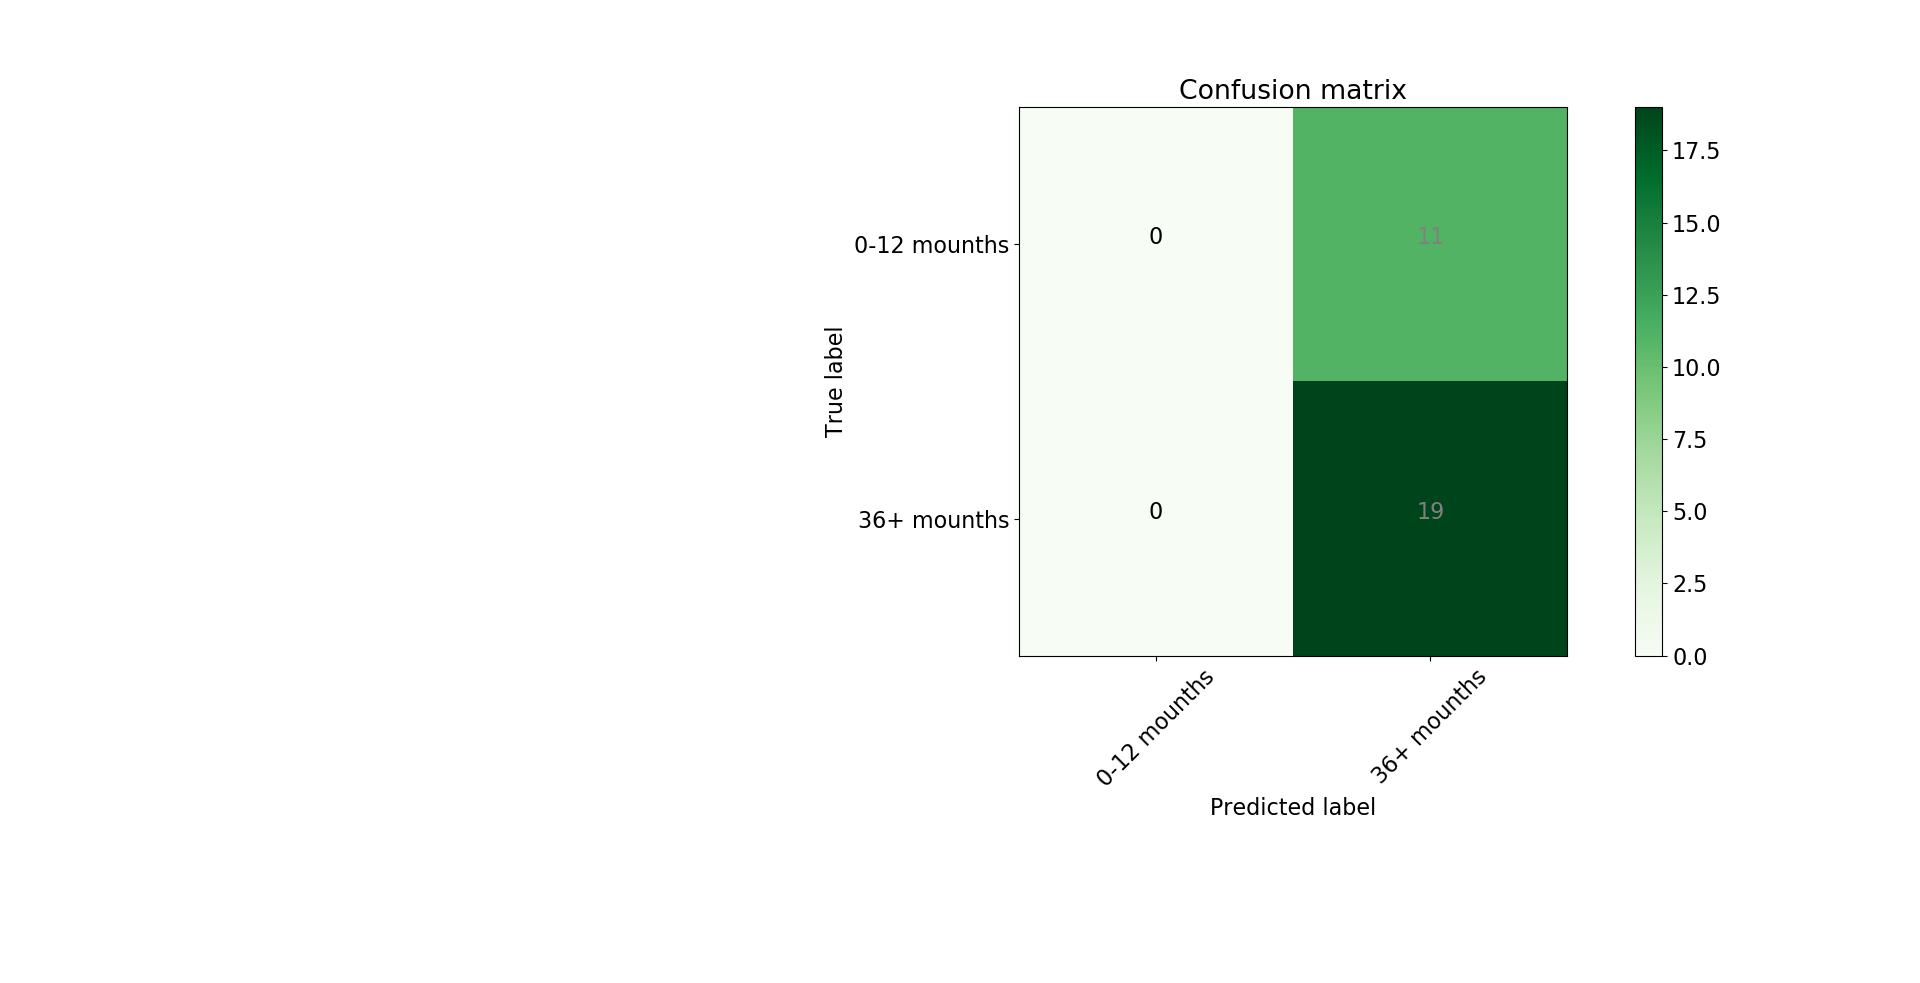
\includegraphics[width=\textwidth]{figures/epain2cla}
    \caption{Confusion matrix for classification of pain intensity}
    \label{fig:f2}
  \end{subfigure}
  \caption{Confusion matrices for combined representation testing}
\end{figure}



\begin{table}[H]
\centering
\begin{tabular}{|p{2cm}|p{2.2cm}|p{2.2cm}|p{2.2cm}|p{2cm}|p{2cm}|}
\hline
Classes          & Accuracy (\%) & Sensitivity (\%) & Specificity (\%) & PPV (\%) & NPV (\%) \\ \hline
Symptom Duration &                    &                      &                       &               &               \\ \hline
Pain intensity   &                    &                      &                       &               &               \\ \hline
\end{tabular}
\label{my-label}
\caption{My caption}
\end{table}

\end{document}
